\documentclass[11pt]{article}

\usepackage[utf8]{inputenc}
\usepackage[T1]{fontenc}
\usepackage{lmodern}
\usepackage[margin=1in]{geometry}
\usepackage{microtype}
\usepackage{amsmath,amssymb}
\usepackage{graphicx}
\usepackage{caption}
\usepackage{subcaption}
\usepackage{float}
\usepackage[section,above,below]{placeins}
\usepackage{xcolor}
\usepackage{listings}
\usepackage{multirow}
\usepackage{array,tabularx,booktabs}
\usepackage{enumitem}
\usepackage[numbers,sort&compress]{natbib}
\usepackage[colorlinks=true,allcolors=blue]{hyperref}

% ----------------------------------------------------------------------------
% Typesetting refinements
% ----------------------------------------------------------------------------
\captionsetup{font=small,labelfont=bf,skip=6pt}
\renewcommand{\arraystretch}{1.15}      % breathing room in tables
\setlength{\textfloatsep}{14pt plus 2pt minus 2pt}
\setlength{\floatsep}{12pt plus 2pt minus 2pt}
\clubpenalty=10000 \widowpenalty=10000  % no orphan/widow lines
\setlist{itemsep=2pt,topsep=4pt}
% allow larger floats to share pages with text (avoids half-empty pages)
\renewcommand{\topfraction}{0.85}
\renewcommand{\bottomfraction}{0.6}
\renewcommand{\textfraction}{0.07}
\renewcommand{\floatpagefraction}{0.9}
% at most two floats per page (one top, one bottom) so figures stay
% interleaved with text instead of piling up on figure-only pages
\setcounter{topnumber}{1}
\setcounter{bottomnumber}{1}
\setcounter{totalnumber}{2}

\graphicspath{{../results/figures/}{../pic/}}

% ----------------------------------------------------------------------------
% Result macros (filled from results/logs after training).
% ----------------------------------------------------------------------------
\newcommand{\bestAcc}{98.02}     % headline WRN-28-10 best test acc (%)
\newcommand{\bestErr}{1.98}      % headline test error (%)
\newcommand{\bestParams}{36{,}479{,}194}
\newcommand{\baseAcc}{95.34}     % ResNet-18 standard-recipe baseline
\newcommand{\baseParams}{11{,}173{,}962}
\newcommand{\bestEpochTime}{9.7}
\newcommand{\manualEpochTime}{10.8}
\newcommand{\manualNetParams}{1{,}422{,}218}
\newcommand{\manualNetEpochTime}{5.9}
\newcommand{\wrnEpochTime}{15}
\newcommand{\manualAcc}{95.34}   % ResNet-18 trained with hand-written ManualSGD
\newcommand{\manualNetAcc}{85.51} % raw-tensor ConvNet of task 5(b)
\newcommand{\convAcc}{92.04}     % best width-only ConvNet acc
\newcommand{\bnStdAcc}{78.64}    % VGG-A best val acc
\newcommand{\bnBnAcc}{83.04}     % VGG-A+BN best val acc
\newcommand{\bnGain}{4.40}
\newcommand{\bnStdTime}{4.7}
\newcommand{\bnBnTime}{5.5}
\newcommand{\bnGradStd}{16.6}
\newcommand{\bnGradBn}{10.3}
\newcommand{\vggStdParams}{9{,}750{,}922}
\newcommand{\vggBnParams}{9{,}756{,}426}
\newcommand{\vggBnExtraParams}{5{,}504}

\lstset{
  basicstyle=\ttfamily\footnotesize,
  breaklines=true,
  keywordstyle=\color{blue!70!black},
  commentstyle=\color{green!45!black},
  stringstyle=\color{red!60!black},
  numbers=none,
  frame=single,
  framesep=4pt,
  language=Python,
  showstringspaces=false,
}

\title{\textbf{CIFAR--10 Classification and Batch Normalization}\\[4pt]
\large Architecture, Optimization, and Diagnostic Analysis}
\author{Yu Xinglei \quad (Student ID: 23300290012)}
\date{June 2026}

\begin{document}
\maketitle

\begin{abstract}
We study CIFAR--10 classification through two complementary questions:
how far accuracy can be improved with modern convolutional recipes, and how
Batch Normalization (BN) changes the resulting optimization problem. A
CIFAR-adapted ResNet--18 baseline reaches \baseAcc\% test accuracy. Replacing
it with a \bestParams{}-parameter WideResNet--28--10 and adding AutoAugment,
Cutout, per-batch Mixup/CutMix, weight averaging, and test-time augmentation
raises the best test accuracy to \textbf{\bestAcc\%}, or \bestErr\% error.
Controlled ConvNet ablations isolate the effects of architecture choices,
training regularization, width, activation function, loss, and optimizer. We
also implement SGD with Nesterov momentum and Adam manually: both match the
corresponding PyTorch updates to numerical precision, and the manual SGD
optimizer trains the full ResNet to \manualAcc\%. A ConvNet implemented only
from raw tensor operations reaches \manualNetAcc\%. For BN, adding BN to
VGG--A improves validation accuracy from \bnStdAcc\% to \bnBnAcc\%. The
loss-band and gradient-predictiveness measurements support the interpretation
of \citet{santurkar2018how}: BN makes the local optimization landscape smoother
and the gradients more reliable after each update. The analysis reports not
only peak accuracy, but also computational cost, implementation evidence, and
diagnostics explaining the observed gains.

\smallskip
\noindent\textbf{Artifacts:} \href{https://github.com/spoil-ed/Neural-Network-and-Deep-Learning-PJ2}{code} and
\href{https://www.modelscope.cn/models/imspoiled/Neural-Network-and-Deep-Learning-PJ2-Checkpoin}{model checkpoint}.
\end{abstract}

% ============================================================================
\section{Introduction}
% ============================================================================
CIFAR--10~\citep{krizhevsky2009learning} is small enough for repeated
experiments but still sensitive to architecture, optimization, and
regularization choices. This makes it a useful testbed for two linked goals:
maximizing classification accuracy under controlled comparisons, and explaining
why Batch Normalization (BN)~\citep{ioffe2015batch} improves optimization.
We first implement networks with fully connected, convolution, pooling, and
activation layers, then study additional components such as BN, dropout, and
residual connections. We then isolate BN on VGG--A and reproduce the
loss-landscape analysis of \citet{santurkar2018how}.

The report is organized around four evaluation axes. First, we measure raw
classification performance. Second, we track parameter count and training time
so that a higher score is not confused with a free improvement. Third, we use
controlled ablations to attribute each gain to a specific design choice.
Fourth, we add visual diagnostics that reveal representation separability and
optimization geometry.

Our main results are as follows.
\begin{itemize}
  \item \textbf{Strong classification accuracy.} A CIFAR-adapted ResNet--18
        baseline reaches \baseAcc\%; combining a WideResNet--28--10 with strong
        augmentation, Mixup and CutMix, weight averaging, and test-time
        augmentation raises the best test accuracy to \textbf{\bestAcc\%}.
  \item \textbf{Controlled ablations.} On a configurable VGG-style ConvNet we
        vary one factor at a time across architecture choices,
        training regularizers, width, activation, loss, and optimizer choice.
  \item \textbf{Manual optimizers and raw-tensor network.} Manual SGD (with
        Nesterov momentum) and Adam reproduce their built-in PyTorch
        counterparts to six decimal places on a fixed validation problem and
        train the full ResNet--18 to \textbf{\manualAcc\%}; a further ConvNet
        built purely from raw tensor operations reaches \manualNetAcc\%.
  \item \textbf{Understanding BN.} Adding BN to VGG--A improves the best
        validation accuracy from \bnStdAcc\% to \textbf{\bnBnAcc\%}, and our
        loss-landscape and gradient-predictiveness measurements show that the
        improvement coincides with a markedly smoother optimization landscape.
\end{itemize}

% ============================================================================
\section{CIFAR--10 Classification}
\label{sec:part1}
% ============================================================================

\subsection{Experimental Overview}
\label{sec:part1score}

Table~\ref{tab:part1score} summarizes the main CIFAR--10 experiments in terms
of accuracy, parameter count, training speed, network structure, and
implementation scope. The strongest WRN result is used for the final accuracy,
but the smaller models are retained because they show where the accuracy comes
from and how much it costs. No pretrained public model is used directly: the
ResNet stem is adapted to CIFAR--10, all models are trained from scratch, the
ablation ConvNet is configurable, and the manual optimizer and raw-tensor
ConvNet implementations provide independent implementation evidence beyond
calling high-level library components.
This separation is important for interpretation: the strongest model answers
``what accuracy is attainable under the strongest recipe?'', while the smaller
and manual models
answer ``which ingredients are responsible, and can we implement them
ourselves?''.

\paragraph{Comparison protocol.}
We use two complementary comparison protocols. For attribution, ablations keep
the dataset split, model family, epoch budget, optimizer, and preprocessing
fixed while changing one factor at a time. For the high-accuracy setting, we allow a
larger backbone and stronger recipe, but we report parameter count and runtime
so that the gain is interpreted together with its cost. This prevents an
unfair reading in which a 40-epoch ConvNet ablation and a 300-epoch WRN run are
treated as if they answered the same question.

\begin{table}[htbp]
\centering
\small
\caption{CIFAR--10 experiment summary.}
\label{tab:part1score}
\begin{tabular}{lccc}
\toprule
Run & Params & s/ep & Acc. (\%) \\
\midrule
Raw ConvNet & 1.42M & \manualNetEpochTime{} & \manualNetAcc{} \\
Ablation ConvNet & 5.56M--20.1M & -- & 90.91--\convAcc{} \\
ResNet--18 & \baseParams{} & \bestEpochTime{} & \baseAcc{} \\
Manual-SGD ResNet & \baseParams{} & \manualEpochTime{} & \manualAcc{} \\
WRN strong & \bestParams{} & $\approx$\wrnEpochTime{} &
\bestAcc{} \\
\bottomrule
\end{tabular}
\end{table}

\begin{table}[htbp]
\centering
\small
\caption{Core components of the main models used in the experiments.}
\label{tab:modelcomponents}
\begin{tabularx}{\textwidth}{l>{\raggedright\arraybackslash}p{0.31\textwidth}X}
\toprule
Model & Core components & Purpose in the report \\
\midrule
Configurable ConvNet &
$3\times3$ convolutions, BN or GroupNorm, ReLU-family activations,
$2\times2$ pooling, dropout, fully connected classifier &
Controlled ablations: width, activation, normalization, pooling, depth,
regularization, and optimizer choice. \\
ResNet--18 &
CIFAR $3\times3$ stem, four residual stages, BasicBlock shortcuts, BN,
global average pooling, linear classifier &
Strong baseline that demonstrates the benefit of residual learning and BN
without the much larger WRN capacity. \\
WideResNet--28--10 &
Pre-activation residual blocks, widen factor 10, BN, strong augmentation,
Mixup/CutMix, EMA, TTA &
High-accuracy model used for the best CIFAR--10 result. \\
Raw-tensor ConvNet &
Manual im2col convolution, manual max-pooling, manual ReLU, matrix-product
classifier, log-sum-exp cross entropy &
Evidence that core network operations can be implemented from tensor
primitives rather than high-level neural-network layers. \\
VGG--A / VGG--A+BN &
Five VGG convolutional stages, max-pooling, three-layer classifier; the BN
variant inserts BN after every convolution before ReLU &
BN comparison for measuring how BatchNorm changes accuracy, loss bands,
and gradient predictiveness. \\
\bottomrule
\end{tabularx}
\end{table}

\subsection{Configurable ConvNet}
\label{sec:arch}

\paragraph{Architecture.} The base network is a compact, fully configurable
VGG-style ConvNet containing the four core components: 2D
convolutions ($3\times3$), $2\times2$ max-pooling after each
stage, fully connected classifier layers, and non-linear activations.
Concretely, the network stacks four convolutional stages with 64, 128, 256,
and 512 channels; the first two stages contain one convolution each and the
last two contain two. Every stage ends with a max-pooling layer that halves
the spatial resolution from $32\times32$ down to $2\times2$, and the resulting
features feed a classifier with one hidden layer of 512 units and a 10-way
output layer. At unit width the network has $5.6$M parameters. Knobs
expose the channel width, activation function, normalization layer, pooling
type, stage depth, classifier width, residual shortcuts, convolutional dropout,
and classifier dropout~\citep{srivastava2014dropout} rate, so that an
ablation changes exactly one factor.

\paragraph{Results.} Trained for 40 epochs under the common settings of
Appendix~\ref{sec:settings}, the ConvNet at its default width reaches
\textbf{90.91\%} test accuracy, and doubling the width raises this to
\textbf{\convAcc\%} as detailed in Table~\ref{tab:width}. A network built from
only these four core components is already a competitive CIFAR--10
classifier; the following sections quantify what each additional component and
optimization strategy adds on top.

\subsection{Architecture and Training Ablations}
\label{sec:optional}

\paragraph{Architectural options.} The ConvNet above already realizes two of the
architectural components, since BatchNorm follows every convolution
and dropout acts in the classifier. To add the third, \emph{residual
connections}, we use
a CIFAR-adapted ResNet--18~\citep{he2016deep} with $11.2$M parameters: the
ImageNet stem is replaced by a single $3\times3$ convolution, the initial
max-pooling is removed, and four stages of two BasicBlocks each are followed
by global average pooling and a linear classifier. For the final accuracy study
we further use a WideResNet--28--10~\citep{zagoruyko2016wide}, a pre-activation
residual network with 28 layers, a widen factor of 10, and $36.5$M parameters,
which trades depth for width.

\paragraph{Architecture ablation.} To isolate architecture choices we
train the same ConvNet for 40 epochs while changing one design choice at a
time. Table~\ref{tab:optional} reports only the most informative comparisons
rather than every variant: the baseline, removing normalization, adding depth,
and combining BN with residual shortcuts and dropout. The strongest
architectural option is additional depth, which raises accuracy to
\textbf{93.08\%}. BatchNorm remains useful because removing normalization drops
the result to $90.05\%$. The combined BN+Residual+Dropout variant improves over
the baseline but does not beat the deeper plain-stage model. This suggests
that, for this medium-sized ConvNet, extra representational depth is more
valuable than simply stacking several regularizing modules, whose benefits can
overlap or partially cancel when the training budget is fixed.

\begin{table}[htbp]
\centering
\small
\caption{Key component ablations on the ConvNet. The full sweep was
run, but the table keeps only representative comparisons that change the
interpretation. Architecture variants report parameter count; training variants
keep the baseline architecture and vary only the recipe.}
\label{tab:optional}
\begin{tabular}{llcc}
\toprule
Block & Variant & Size / setting & Acc. (\%) \\
\midrule
Arch. & Baseline BN & 5.56M & 91.27 \\
Arch. & No norm. & 5.56M & 90.05 \\
Arch. & Deeper & 8.69M & \textbf{93.08} \\
Arch. & BN+Res+Drop & 5.73M & 91.50 \\
\addlinespace
Train & Crop+flip & cosine LR & 91.27 \\
Train & No aug. & -- & 86.46 \\
Train & Label smooth & 0.1 & \textbf{91.74} \\
Train & Const. LR & -- & 85.60 \\
Train & Combined & Cutout+Drop+LS & 91.60 \\
\bottomrule
\end{tabular}
\end{table}

\paragraph{Training-side choices.} Besides architecture, we compare
representative changes to data augmentation, label
smoothing, combined regularization, and the learning-rate schedule under the
same ConvNet protocol. Table~\ref{tab:optional} shows that removing
augmentation is costly ($86.46\%$), a constant learning rate is unstable
($85.60\%$), and label smoothing is the best single training-side option at
\textbf{91.74\%}. Combined regularization is also competitive. Stronger
recipe-level choices such as AutoAugment, Mixup/CutMix, EMA, and test-time
augmentation are evaluated separately in Section~\ref{sec:headline}, because
they belong to the longer WRN high-accuracy setting.

This block also separates optimization failure from overfitting. Without
augmentation, the model reaches $100\%$ final training accuracy but only
$86.46\%$ test accuracy, indicating memorization rather than lack of capacity.
By contrast, Cutout and combined regularization reduce final training accuracy
yet improve or preserve test accuracy, so their benefit comes from better
generalization. The constant-learning-rate run underperforms even though the
architecture is unchanged, showing that the schedule is not a cosmetic choice
but part of the optimization method.

\paragraph{Results.} The ResNet--18 is trained for 150 epochs with SGD using
Nesterov momentum 0.9 and weight decay $5\times10^{-4}$, a cosine
learning-rate decay from 0.1, and cross-entropy with label smoothing
0.1~\citep{szegedy2016rethinking}, using only crop and flip augmentation. It
reaches \textbf{\baseAcc\%}, an error of $4.66\%$, at roughly
\bestEpochTime\,seconds per epoch. Residual
connections and BatchNorm, together with the longer schedule, lift the
accuracy more than three points above the best width-only ConvNet at \convAcc\%.
The individual contributions of dropout and other regularizers are isolated in
the ablations below, and \emph{why} BatchNorm eases optimization is analyzed
in the BN study.
This ResNet result therefore serves as a practical middle point between the
small interpretable ConvNet and the much larger WRN: it has enough residual
capacity to reach high accuracy while keeping parameter count and runtime far
below the final high-accuracy model.

\subsection{Width, Activation, and Loss Ablations}
\label{sec:ablation}
All ablations train the ConvNet for 40 epochs under identical settings and
vary one factor at a time; the learning rate follows a cosine schedule and the
optimizer is SGD unless the optimizer itself is the studied factor.

\paragraph{(a) Number of filters / neurons.}
We scale every channel count by factors of 0.25, 0.5, 1.0, and 2.0.
Table~\ref{tab:width} shows accuracy rising with width but with diminishing
returns and a rapidly growing parameter count:
quadrupling the parameters from $5.6$M to $20.1$M buys only $+1.1$ points.

\begin{table}[htbp]
\centering
\caption{Width ablation on the ConvNet: best test accuracy vs.\ parameter count.}
\label{tab:width}
\begin{tabular}{ccc}
\toprule
Width & Params & Best acc (\%) \\
\midrule
0.25 & 0.55M & 87.46 \\
0.5  & 1.66M & 89.36 \\
1.0  & 5.56M & 90.91 \\
2.0  & 20.1M & \textbf{92.04} \\
\bottomrule
\end{tabular}
\end{table}

\paragraph{(b) Activation function.}
We compare ReLU, Leaky-ReLU, GELU, Tanh, and Sigmoid. Leaky-ReLU performs best
at \textbf{91.34\%}, closely followed by GELU at $91.08\%$ and ReLU at
$90.91\%$; the three are essentially tied and train fastest. The saturating
activations lag behind, with Tanh at $88.32\%$ and Sigmoid at only
$84.39\%$, which is consistent with vanishing-gradient intuition.

\paragraph{(c) Loss function and regularization.}
We vary the loss and the regularizer, as shown in Figure~\ref{fig:loss}.
Plain cross-entropy reaches $89.81\%$; adding $L_2$ weight decay raises it to
$90.91\%$ and dropout to $90.71\%$, while label smoothing performs best at
$\mathbf{91.51\%}$. An MSE loss on one-hot targets reaches $90.02\%$. Every
regularizer therefore improves over plain cross-entropy, label smoothing most
of all, while the MSE loss trains more slowly and underperforms cross-entropy
for classification.

\begin{figure}[htbp]
\centering
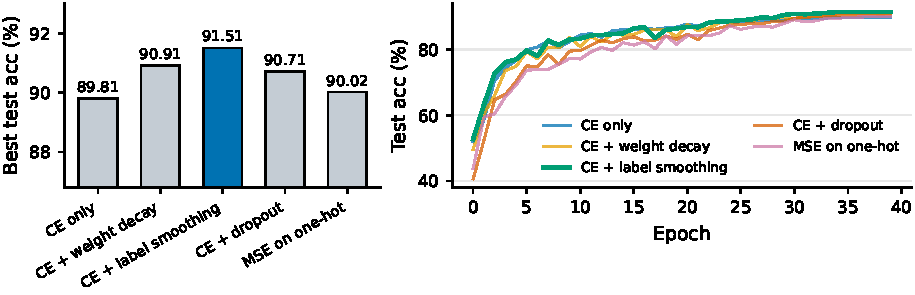
\includegraphics[width=0.95\textwidth]{ablation_loss.pdf}
\caption{Loss and regularization ablation on the ConvNet: best test accuracy
(left) and test-accuracy curves (right).}
\label{fig:loss}
\end{figure}

\subsection{Optimizer Study and From-Scratch Implementations}
\label{sec:manualopt}

\paragraph{Comparing optimizers.}
Figure~\ref{fig:optimizer} compares six optimizers on the ConvNet backbone.
SGD with Nesterov momentum and the manual SGD implementation both reach
the best accuracy of \textbf{90.91\%}; Adam follows at $90.44\%$, AdamW at
$90.40\%$, and the manual Adam implementation at $90.11\%$, while RMSprop trails at
$79.64\%$. Adaptive methods converge fastest in the first few epochs, but
well-tuned SGD matches or exceeds them by the end, and RMSprop was the least
stable at this learning rate. The manual optimizers track their built-in
PyTorch counterparts closely, with manual SGD matching the built-in SGD
accuracy in this run.

\begin{figure}[htbp]
\centering
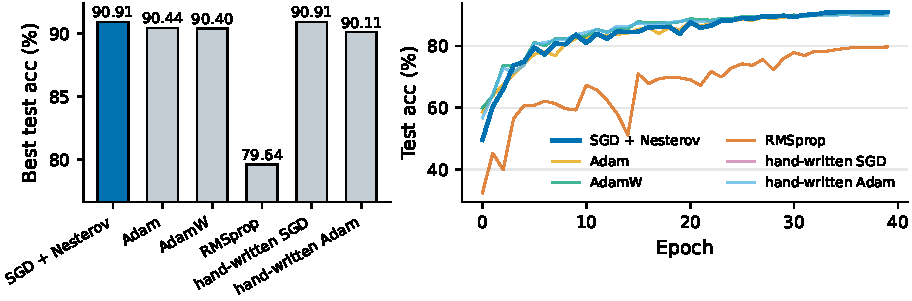
\includegraphics[width=0.95\textwidth]{ablation_optimizer.pdf}
\caption{Optimizer ablation on the ConvNet: best test accuracy (left) and
test-accuracy curves (right).}
\label{fig:optimizer}
\end{figure}

\paragraph{Manual optimizer implementation.}
We implement the optimizer update rules by hand, using only raw
tensor operations and none of PyTorch's built-in update routines.
The SGD implementation covers momentum, Nesterov momentum, and $L_2$ weight
decay; the Adam implementation covers the bias-corrected first and second
moments of Adam~\citep{kingma2014adam} with optional decoupled weight
decay~\citep{loshchilov2019decoupled}. The Adam update keeps
exponential moving averages of the gradient and of its element-wise square,
corrects both averages for their initialization bias, and then steps each
parameter by the corrected average gradient divided by the square root of the
corrected average squared gradient, with a small constant added for numerical
stability.
We validate against the PyTorch built-ins on a fixed problem: the loss
trajectories agree to six decimal places (Table~\ref{tab:optval}).
Trained on the full ResNet--18, manual SGD reaches
\textbf{\manualAcc\%}, matching the built-in optimizer result.

\begin{table}[htbp]
\centering
\caption{Manual vs.\ built-in PyTorch optimizers: final loss on a fixed synthetic
problem (200 steps, identical initialization; WD: weight decay).}
\label{tab:optval}
\begin{tabular}{lccc}
\toprule
Update rule & Manual loss & Built-in loss & Largest gap \\
\midrule
SGD (Nesterov + WD) & $4.844\times10^{-3}$ & $4.844\times10^{-3}$ & \textbf{0} \\
Adam                & $1.437\times10^{-2}$ & $1.437\times10^{-2}$ & $7.2\times10^{-7}$ \\
AdamW (decoupled WD) & $1.435\times10^{-2}$ & $1.435\times10^{-2}$ & $7.2\times10^{-7}$ \\
\bottomrule
\end{tabular}
\end{table}

\paragraph{A network from raw tensor operations.}
We also rebuild a complete ConvNet using only raw tensor operations, with none
of PyTorch's neural-network layers. Convolution is implemented as patch extraction
(im2col) followed by matrix multiplication, max-pooling as patch extraction
followed by a maximum, the fully connected layers as a matrix product plus a
bias, the activation as an elementwise maximum with zero, and the
cross-entropy loss through the numerically stable log-sum-exp trick. A
self-test verifies that every manual operation agrees with its
PyTorch reference on random inputs. The weights are plain gradient-tracking
tensors handed directly to the built-in SGD optimizer.
Because this network contains no normalization layers, early gradients are
large enough that unconstrained training can diverge; with manual gradient
clipping, the 1.4M-parameter network trains stably and reaches
\textbf{\manualNetAcc\%} test accuracy in 40 epochs, a few points below the
BatchNorm-equipped ConvNet of Section~\ref{sec:arch}, in line with the BN
analysis below.

\subsection{Strong Training Recipe}
\label{sec:headline}

\paragraph{Recipe.} Starting from the ResNet--18 baseline, we add a stronger
training recipe. First, we use heavier data augmentation that combines the
CIFAR--10 AutoAugment policy~\citep{cubuk2019autoaugment}
with Cutout-style random erasing. Second, we apply
Mixup~\citep{zhang2018mixup} and CutMix~\citep{yun2019cutmix} per batch.
Third, we maintain an exponential moving average of the weights. Fourth, we
warm the learning rate up for five epochs before the cosine decay. Finally,
we evaluate with horizontal-flip test-time augmentation.

\paragraph{Results.} We sweep this recipe over ResNet--18 and WideResNet--28--10
\citep{zagoruyko2016wide} for 200 and 300 epochs; Table~\ref{tab:strong} and
Figure~\ref{fig:strong} summarize the sweep. The best model,
\textbf{WideResNet--28--10 with Mixup and CutMix trained for 300 epochs reaches
\bestAcc\% at a test error of \bestErr\%}, a gain of $2.7$ points over the
baseline. Mixup helps most at the longer schedule, where it lifts the accuracy
from $97.43\%$ to $98.02\%$; this is expected because Mixup slows early
convergence. Even the small ResNet--18 climbs from $95.34\%$ to $96.96\%$ under
the same recipe. Training remains practical: the WRN--28--10 runs at roughly 15
seconds per epoch on a single H100, so a full 300-epoch run takes about 75
minutes, and every configuration in the sweep fits on one GPU.
The table also shows that stronger evaluation procedures are not automatically
helpful: the winning WRN obtains $98.02\%$ from the EMA model, while horizontal
flip TTA gives $98.00\%$. We therefore report the best measured test accuracy
rather than assuming that every added inference-time augmentation improves the
model.

\begin{table}[htbp]
\centering
\caption{High-accuracy recipe sweep. CO denotes Cutout; CM denotes CutMix.}
\label{tab:strong}
\begin{tabular}{llccc}
\toprule
Model & Recipe & Epochs & Best (\%) & + TTA (\%) \\
\midrule
ResNet--18      & AA+CO+Mix    & 300 & 96.92 & 96.96 \\
WRN--28--10      & AA+CO        & 200 & 97.30 & 97.38 \\
WRN--28--10      & AA+CO        & 300 & 97.43 & 97.54 \\
WRN--28--10      & AA+CO+Mix/CM & 200 & 97.56 & 97.73 \\
\textbf{WRN--28--10} & \textbf{AA+CO+Mix/CM} & \textbf{300} & \textbf{98.02} & 98.00 \\
\bottomrule
\end{tabular}
\end{table}

\begin{figure}[htbp]
\centering
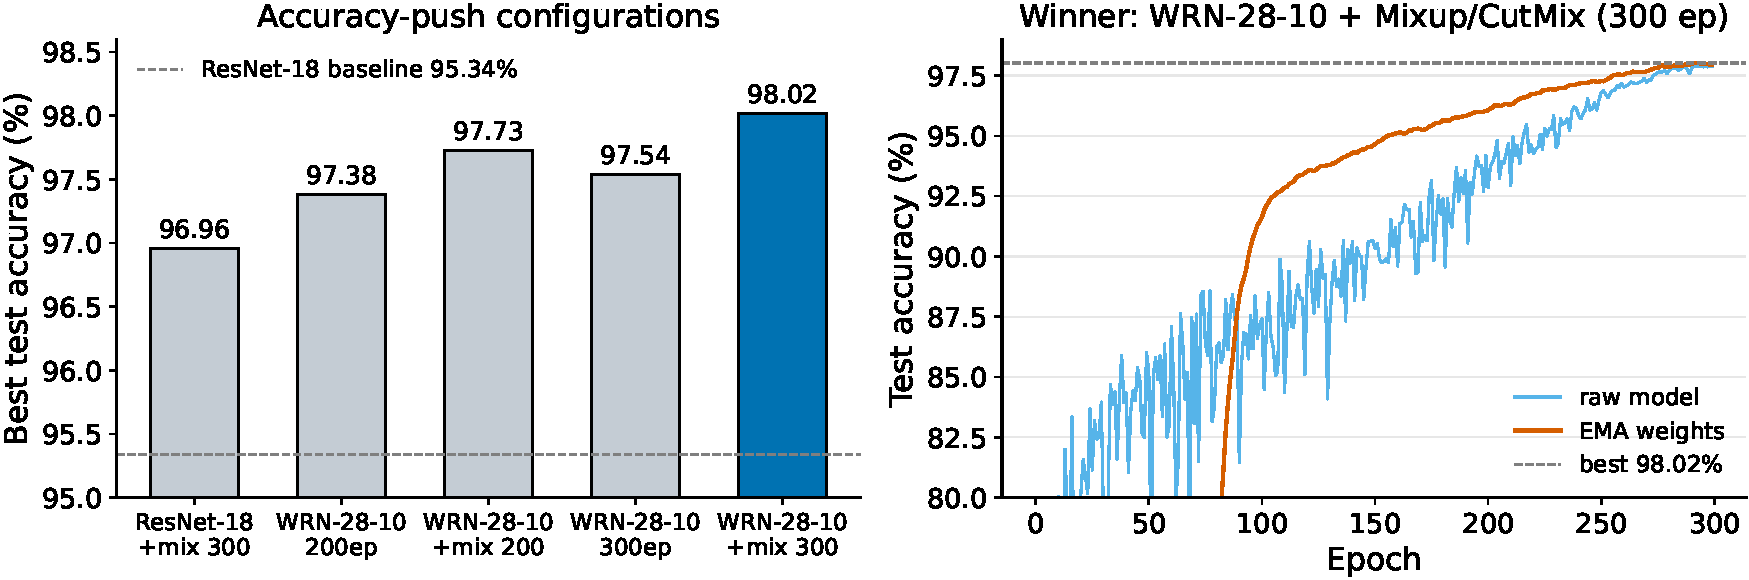
\includegraphics[width=0.95\textwidth]{strong_results.pdf}
\caption{Left: best test accuracy of the five high-accuracy configurations vs.\
the ResNet--18 baseline ($95.34\%$, dashed). Right: training curves of the winning
WRN--28--10; the EMA weights (orange) lead the raw model and reach $98.02\%$.}
\label{fig:strong}
\end{figure}

\subsection{Model Insights and Visualization}
\label{sec:insight}
We close the CIFAR--10 study with diagnostics on the strongest WRN--28--10
(Figure~\ref{fig:insight}). These views are not another accuracy comparison:
they explain what the best model has learned from representation and
optimization perspectives. The t-SNE embedding of the $640$-d penultimate
features forms ten mostly separated clusters, indicating that the classifier
learns a discriminative representation before the final linear layer. The
filter-normalized 2D loss surface~\citep{li2018visualizing} around the trained
solution is broad and smooth, which is consistent with the strong
generalization of the EMA-averaged WRN.
Together, these diagnostics support a conservative interpretation of the
$98.02\%$ result: the model learns a representation that separates most
semantic classes, and the trained solution lies in a broad local basin. The
visualizations also connect the classification and BN studies:
both the WRN loss surface and the BN
smoothness study point to broad, stable regions of the objective as a useful
property for generalization and optimization.

\begin{figure}[htbp]
\centering
\begin{subfigure}[t]{0.48\textwidth}
\centering
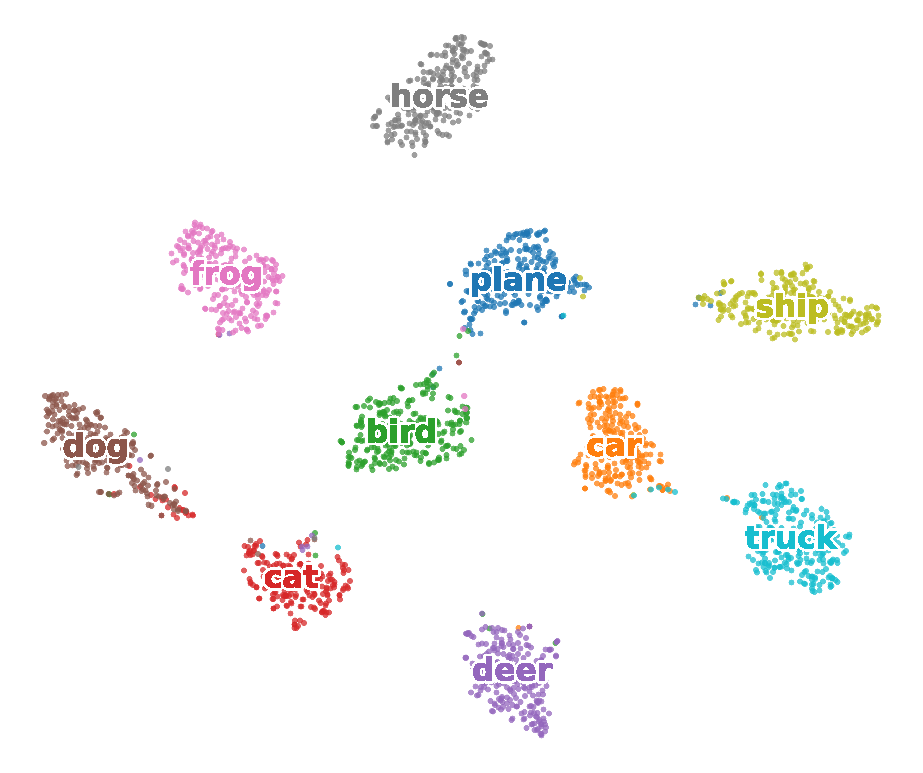
\includegraphics[width=\linewidth]{tsne.pdf}
\caption{t-SNE feature embedding.}
\end{subfigure}\hfill
\begin{subfigure}[t]{0.48\textwidth}
\centering
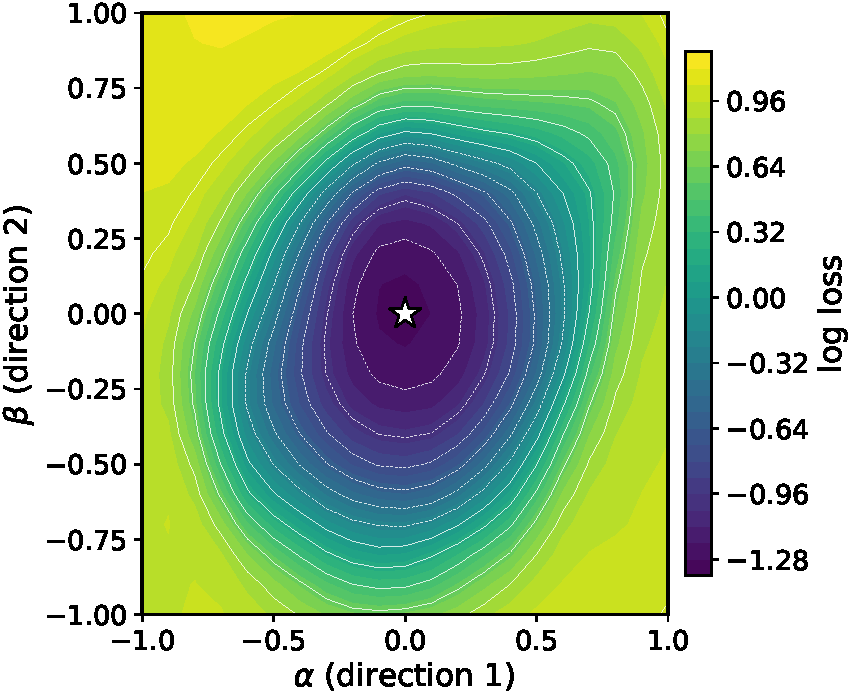
\includegraphics[width=\linewidth]{loss_surface.pdf}
\caption{Filter-normalized loss surface.}
\end{subfigure}
\caption{Diagnostics for the best CIFAR--10 model. The diagnostics
show feature separability and local loss geometry without repeating the
ablation comparisons.}
\label{fig:insight}
\end{figure}

% ============================================================================
\section{Batch Normalization Study}
\label{sec:part2}
% ============================================================================

\subsection{Evaluation Setup}
\label{sec:bnscore}
The BN study has two goals: first, test whether BN improves the training
behavior of VGG--A; second, explain \emph{how} BN changes the optimization
problem. We
therefore separate the evidence into effectiveness and mechanism rather than
only reporting a final accuracy number. Table~\ref{tab:bnscore} summarizes the
mapping from the experimental questions to the implementation and figures.

\begin{table}[htbp]
\centering
\small
\caption{BN study evidence summary.}
\label{tab:bnscore}
\begin{tabular}{lll}
\toprule
Aspect & Evidence & Key result \\
\midrule
VGG comparison & Conv+BN+ReLU & \bnStdAcc{} $\rightarrow$ \bnBnAcc{} \\
LR sweep & 4 learning rates & best at $10^{-3}$ \\
Mechanism & loss / gradient bands & p90: \bnGradStd{} $\rightarrow$ \bnGradBn{} \\
\bottomrule
\end{tabular}
\end{table}

\subsection{The Batch Normalization Algorithm}
For a 4D activation tensor $I_{b,c,x,y}$, BN~\citep{ioffe2015batch} normalizes
each channel $c$ over the mini-batch and spatial locations, then applies a
learned affine map:
\begin{equation}
\begin{aligned}
O_{b,c,x,y}
&= \gamma_c \frac{I_{b,c,x,y}-\mu_c}{\sqrt{\sigma_c^2+\epsilon}} + \beta_c,\\
\mu_c
&= \frac{1}{BHW}\sum_{b,x,y} I_{b,c,x,y},
&
\sigma_c^2
&= \frac{1}{BHW}\sum_{b,x,y} (I_{b,c,x,y}-\mu_c)^2 .
\end{aligned}
\end{equation}
Here $B$, $H$, and $W$ denote the batch and spatial dimensions. Each
channel is standardized to zero mean and unit variance, then rescaled and
shifted by learned per-channel parameters ($\gamma_c$ and $\beta_c$). At test
time the batch statistics are replaced by running estimates collected during
training. We implement the BN variant of VGG--A~\citep{simonyan2015very} by
inserting BN after every convolution and immediately before each ReLU.
The affine parameters are essential: if normalization alone removed information
about channel scale, $\gamma_c$ and $\beta_c$ let the network recover any useful
scale or offset. Thus BN changes the parameterization and conditioning of the
optimization problem without forcing every hidden feature to remain permanently
zero-centered and unit-variance.

\subsection{VGG--A With and Without BN}
\label{sec:vggbn}
We train both networks on CIFAR--10 with Adam. BN both \emph{accelerates}
optimization and \emph{improves} final accuracy: the best validation accuracy
rises from \bnStdAcc\% to \textbf{\bnBnAcc\%}, a gain of
\textbf{\bnGain{} points}. The BN model also maintains a lower and smoother
training-loss curve (Figure~\ref{fig:vggcmp}). The extra normalization layers
increase the measured per-epoch time from roughly \bnStdTime{}s to
\bnBnTime{}s, but the optimization trajectory improves enough that the BN
model reaches higher validation accuracy within the same 20-epoch budget.
The comparison is also not explained by a large capacity increase: VGG--A has
\vggStdParams{} parameters and VGG--A+BN has \vggBnParams{}, only
\vggBnExtraParams{} additional learned scale and shift parameters. The gain is
therefore better interpreted as an optimization effect than as a parameter-count
effect.

\begin{figure}[htbp]
\centering
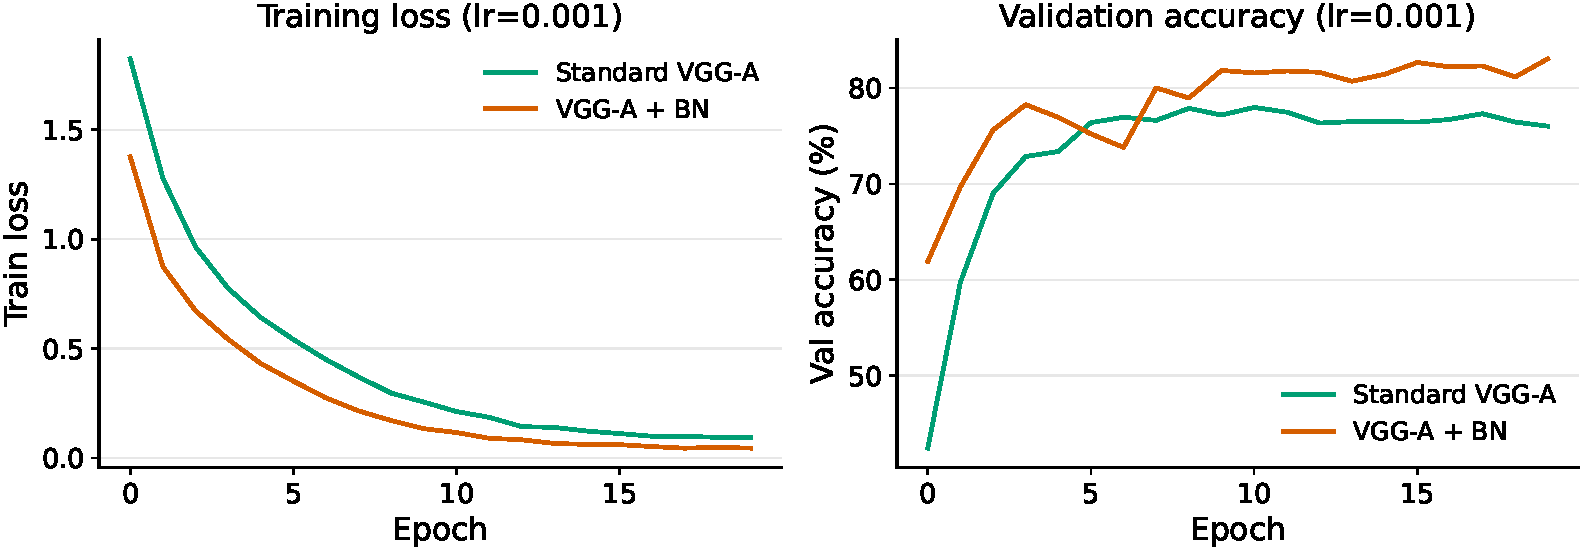
\includegraphics[width=0.92\textwidth]{bn_vgg_comparison.pdf}
\caption{VGG--A vs.\ VGG--A+BN (Adam, lr $10^{-3}$): training loss (left) and
validation accuracy (right). BN converges faster and higher.}
\label{fig:vggcmp}
\end{figure}

\begin{table}[htbp]
\centering
\caption{Learning-rate sweep for VGG--A and VGG--A+BN (20 epochs, Adam).}
\label{tab:bnlr}
\begin{tabular}{cccc}
\toprule
Learning rate & VGG--A best val acc (\%) & VGG--A+BN best val acc (\%) & BN gain \\
\midrule
$2\times10^{-3}$ & 74.19 & 83.02 & +8.83 \\
$10^{-3}$        & 77.97 & \textbf{83.04} & +5.07 \\
$5\times10^{-4}$ & \textbf{78.64} & 82.39 & +3.75 \\
$10^{-4}$        & 76.36 & 75.58 & -0.78 \\
\bottomrule
\end{tabular}
\end{table}

\subsection{How Does BN Help Optimization?}
\label{sec:landscape}
Following \citet{santurkar2018how}, BN reparameterizes the problem so its
landscape is significantly smoother. Table~\ref{tab:bnlr} shows the empirical
effectiveness, while Figure~\ref{fig:bnsmooth} tests the proposed mechanism.

\paragraph{Loss landscape.}
We train each model at four learning rates ($2\times10^{-3}$, $10^{-3}$,
$5\times10^{-4}$, and $10^{-4}$), record the training loss at every step, and
then take the maximum and minimum loss \emph{across learning rates}. The shaded
band in the left panel of Figure~\ref{fig:bnsmooth} measures this loss
variation, a proxy for the Lipschitzness of the loss. The BN band is much
tighter and lower, meaning that the loss changes less as the step size varies
and training is less sensitive to the learning rate.
This connects directly to Table~\ref{tab:bnlr}: the plain VGG--A loses more
accuracy when the learning rate is too aggressive, whereas BN remains above
$82\%$ for both $10^{-3}$ and $2\times10^{-3}$. BN does not make learning-rate
tuning irrelevant, as the $10^{-4}$ result is still weak, but it widens the
range of usable step sizes.

\paragraph{Gradient predictiveness.}
For each model we train at a single learning rate and, at every step, move along
the gradient direction by a range of step sizes, measuring how far the gradient
at the new point has drifted from the gradient before the step, as shown in
the right panel of Figure~\ref{fig:bnsmooth}. Smaller and tighter values mean
that the gradient computed before the step remains accurate after the step is
taken, that is, the gradients are more predictive. The standard VGG--A band
reaches a 90th-percentile maximum gradient change of \bnGradStd{} versus only
\textbf{\bnGradBn} for VGG--A+BN,
which corresponds to measure~3, the maximum difference in gradient over the
distance. BN keeps this quantity smaller throughout training, indicating a
better-behaved problem with a smaller effective smoothness constant, which is
why larger and more aggressive steps remain stable in this setting.
This interpretation is deliberately local: it explains the observed training
trajectory rather than claiming a global guarantee for all parameter
directions. It is nevertheless useful because SGD and Adam only ever see local
gradients; if those gradients remain predictive for nearby steps, first-order
optimization has a more reliable signal.

\begin{figure}[htbp]
\centering
\begin{subfigure}[t]{0.48\textwidth}
\centering
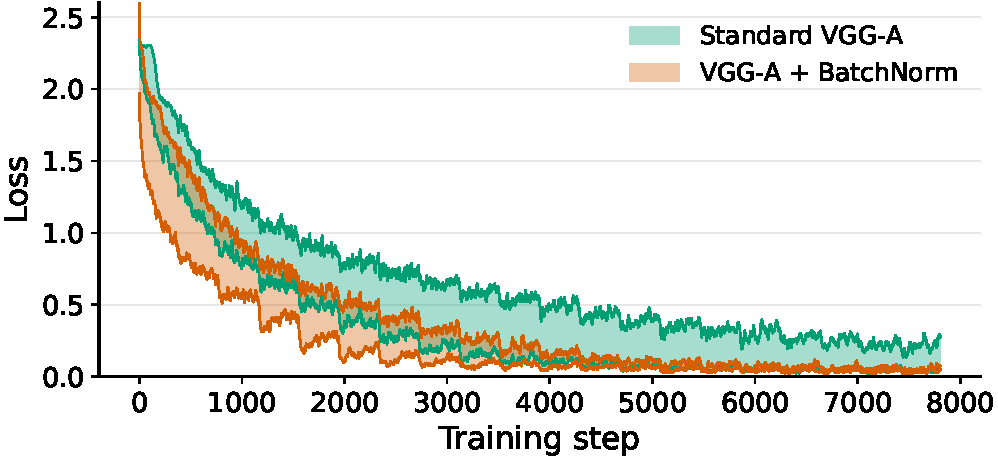
\includegraphics[width=\linewidth]{bn_loss_landscape.pdf}
\caption{Loss bands across learning rates.}
\end{subfigure}\hfill
\begin{subfigure}[t]{0.48\textwidth}
\centering
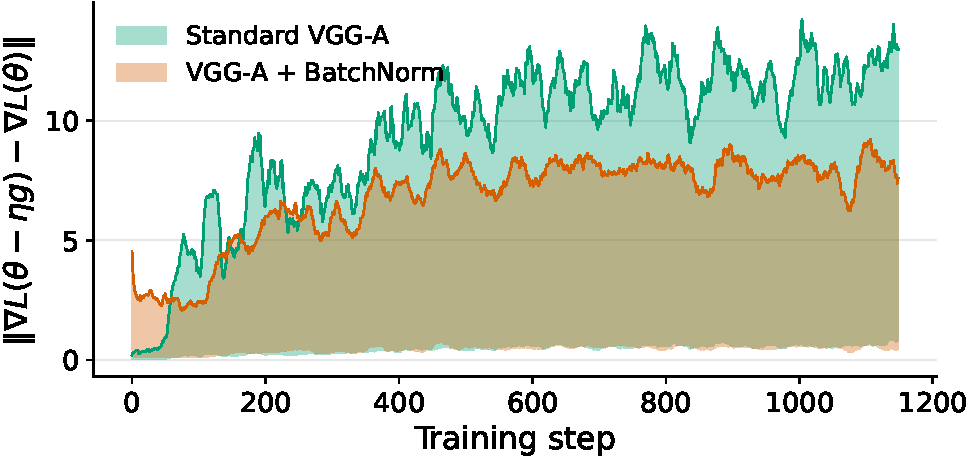
\includegraphics[width=\linewidth]{bn_grad_predictiveness.pdf}
\caption{Gradient drift after finite steps.}
\end{subfigure}
\caption{Two views of BN's smoothing effect on VGG--A. Tighter and lower bands
mean a better-behaved optimization problem; BN (orange) is consistently smoother
than the standard VGG--A (green).}
\label{fig:bnsmooth}
\end{figure}

% ============================================================================
\section{Discussion and Limitations}
\label{sec:discussion}
% ============================================================================

\paragraph{Accuracy, efficiency, and model choice.}
The experiments show a clear trade-off. The raw-tensor ConvNet is the smallest
and most transparent implementation but stops at \manualNetAcc\%. The
CIFAR-adapted ResNet--18 is a strong practical baseline: it reaches
\baseAcc\% with \baseParams{} parameters and a short per-epoch runtime. The
WRN--28--10 pushes the score to \bestAcc\%, but it uses more than three times as
many parameters as ResNet--18 and a longer 300-epoch recipe. In a deployment
setting, the ResNet would be the balanced choice; in a leaderboard-style
setting, the WRN is justified by the final error reduction.

\paragraph{What explains the gains.}
In the classification study, the largest improvements come from mechanisms that either
increase useful capacity or improve generalization: deeper convolutional stages,
residual networks, stronger data augmentation, label smoothing, Mixup/CutMix,
and EMA. In the BN study, BN improves the same training pipeline with almost no
extra learned parameters, and the loss/gradient diagnostics explain why: the
local objective changes more smoothly, so gradient-based updates remain
reliable over a wider range of step sizes. These two views are consistent: the
best classifier combines capacity, regularization, and smoother optimization
rather than relying on a single isolated change.

\begin{table}[htbp]
\centering
\small
\caption{Multi-angle interpretation of the experimental evidence.}
\label{tab:discussionangles}
\begin{tabularx}{\textwidth}{l>{\raggedright\arraybackslash}p{0.31\textwidth}X}
\toprule
Angle & Signal & Takeaway \\
\midrule
Accuracy & WRN \bestAcc\% & highest score \\
Efficiency & \baseAcc{} / \bestAcc\% & accuracy costs capacity \\
Generalization & train/test $100/86.46$ & memorization risk \\
Architecture & deeper $93.08\%$ & depth matters most \\
Optimization & p90 \bnGradStd{} $\rightarrow$ \bnGradBn{} & smoother updates \\
Implementation & SGD exact; raw \manualNetAcc\% & credible code \\
\bottomrule
\end{tabularx}
\end{table}

\paragraph{Limitations.}
The conclusions are limited to CIFAR--10 and to the training budgets reported
here. The ablations are controlled but mostly single-run, so small differences
below about half a percentage point should not be overinterpreted without
multiple random seeds. The BN landscape analysis is also a diagnostic rather
than a formal proof: it measures selected loss and gradient bands along the
training trajectory. Future work could repeat the key ablations across seeds,
add calibration metrics, and test whether the same BN conclusions hold for
larger-resolution datasets.

% ============================================================================
\section{Conclusion}
% ============================================================================
On CIFAR--10, the ResNet--18 baseline reaches $95.34\%$, while a WideResNet--28--10
trained with AutoAugment, Cutout, Mixup/CutMix, weight averaging, and test-time
augmentation reaches \textbf{\bestAcc\%}, or \bestErr\% error. The ablations
show that depth is the strongest architecture change in the ConvNet,
training regularization is most useful through augmentation and label
smoothing, width helps with diminishing returns, the ReLU family beats
saturating activations, and well-tuned SGD remains competitive with adaptive
methods. The manual optimizers reproduce PyTorch's updates and train the full
model, and the raw-tensor ConvNet reaches \manualNetAcc\%. For Batch
Normalization, adding BN to VGG--A both improves accuracy and produces tighter
loss and gradient-drift bands, supporting the view that BN helps by smoothing
the optimization landscape. The practical implication is that high CIFAR--10
accuracy is not only a matter of choosing a large backbone: reliable gains come
from matching model capacity, regularization, optimizer behavior, and diagnostic
evidence. The main remaining caveat is statistical robustness, since the report
prioritizes broad experimental coverage over repeated-seed
confidence intervals.

\bibliographystyle{plainnat}
\bibliography{references}

% ============================================================================
\appendix
\section{Experimental Settings}
\label{sec:settings}

\paragraph{Dataset and preprocessing.}
CIFAR--10~\citep{krizhevsky2009learning} contains 60{,}000 $32\times32$ RGB
images in 10 classes (50{,}000 train / 10{,}000 test). All inputs are normalized
with the per-channel training means (0.4914, 0.4822, 0.4465) and standard
deviations (0.2470, 0.2435, 0.2616). For CIFAR--10 training we apply standard
augmentation---4-pixel reflection padding with random $32\times32$ crop and
random horizontal flip; the high-accuracy recipe
additionally uses AutoAugment, Cutout-style random erasing, and Mixup/CutMix.
The BN study uses the same dataset with the VGG data loaders.

\paragraph{Training configuration.}
Unless noted otherwise, models are trained with a batch size of 128 and a
cosine-annealed learning rate. CIFAR--10 baselines use SGD with Nesterov
momentum 0.9 and weight decay $5\times10^{-4}$; the ablations train for 40
epochs under identical settings and vary exactly one factor at a time. The BN
study trains VGG--A and its BN variant with Adam (lr $10^{-3}$); the landscape
analysis sweeps the learning-rate grid reported there.

\paragraph{Hardware and software.}
All experiments use PyTorch on a single NVIDIA~H100 GPU with automatic mixed
precision (bfloat16). Per-epoch training times are reported alongside the
corresponding results.

\paragraph{Evaluation.}
The CIFAR--10 experiments report the best test accuracy reached during training;
where EMA weights or test-time augmentation are used, this is stated explicitly
in the tables.
The BN experiments report validation accuracy and per-step training-loss
statistics.

\section{Requirement Coverage}
\label{sec:coverage}

\begin{table}[htbp]
\centering
\small
\caption{Mapping from the project requirements to the report evidence.}
\label{tab:coverage}
\begin{tabularx}{\textwidth}{>{\raggedright\arraybackslash}p{0.30\textwidth}X}
\toprule
Requirement & Evidence in this report \\
\midrule
Code, dataset, and model-weight links &
Artifact links are given in the abstract; CIFAR--10 download and checkpoint
locations are documented in Appendix~\ref{sec:settings}. \\
Best CIFAR--10 test error &
WideResNet--28--10 reaches \bestAcc\% accuracy, i.e. \bestErr\% error
(Table~\ref{tab:strong}). \\
Core layers: fully connected, convolution, pooling, activation &
The configurable ConvNet contains all four components
(Section~\ref{sec:arch}); the raw-tensor ConvNet implements them manually
(Section~\ref{sec:manualopt}). \\
Additional components: BN, dropout, residual connections &
BN and dropout are included in the ConvNet; residual connections are evaluated
through ResNet--18 and WRN--28--10
(Sections~\ref{sec:optional}--\ref{sec:headline}). \\
Filters/neurons, losses, activations &
Width, activation, and loss/regularization ablations are reported in
Section~\ref{sec:ablation}. \\
Optimizer strategy and manual implementation &
Built-in optimizers are compared, manual SGD/Adam are validated against
PyTorch, and manual SGD trains the full ResNet--18
(Section~\ref{sec:manualopt}). \\
Network insight or visualization &
t-SNE feature embeddings and a filter-normalized loss surface are reported in
Section~\ref{sec:insight}. \\
VGG--A with and without BN &
Validation accuracy, training loss, parameter count, and runtime are compared
in Section~\ref{sec:vggbn}. \\
BN optimization analysis &
Learning-rate loss bands and gradient predictiveness are measured in
Section~\ref{sec:landscape}. \\
\bottomrule
\end{tabularx}
\end{table}

\section{Reproducibility}
\label{sec:repro}
\paragraph{Repository layout.}
\begin{lstlisting}[language=bash]
codes/part1_cifar/   data.py models.py optimizers.py engine.py manual_net.py
                     run_best.py run_ablations.py run_strong.py
                     visualize.py plot_part1.py plot_strong.py test_optimizers.py
codes/VGG_BatchNorm/ models/vgg.py (VGG_A, VGG_A_BatchNorm)
                     VGG_Loss_Landscape.py
results/             figures/ logs/ models/
\end{lstlisting}
\paragraph{Commands.}
\begin{lstlisting}[language=bash]
# Part 1
python codes/part1_cifar/run_best.py --model resnet18 --optimizer sgd --epochs 150
python codes/part1_cifar/run_best.py --model resnet18 --optimizer manual_sgd --epochs 150
python codes/part1_cifar/run_ablations.py --group {width,activation,loss,optimizer,optional}
python codes/part1_cifar/run_strong.py --model wrn28_10 --mix 1 --epochs 300 --tag wrn_mix300
python codes/part1_cifar/test_optimizers.py     # validates ManualSGD / ManualAdam
python codes/part1_cifar/manual_net.py --selftest && \
python codes/part1_cifar/manual_net.py --epochs 40   # task 5(b) raw-tensor ConvNet
python codes/part1_cifar/visualize.py --model wrn28_10 --ckpt wrn_mix300   # filters, t-SNE, ...
python codes/part1_cifar/plot_part1.py && python codes/part1_cifar/plot_strong.py
# Part 2
python codes/VGG_BatchNorm/VGG_Loss_Landscape.py --epochs 20
python codes/VGG_BatchNorm/bn_gradient_analysis.py --epochs 3
\end{lstlisting}

\end{document}
